\section{Casi d'uso}

\subsection{Attori}
In un diagramma dei casi d'uso, gli attori rappresentano le entità esterne che interagiscono con il prodotto \textit{Etherless}. Essi si possono distinguere in due categorie:
\begin{itemize}
	\item \textbf{Attori primari:} coinvolti nell'esecuzione dei casi d'uso, interagiscono con il servizio per soddisfare i propri bisogni;
	\item \textbf{Attori secondari:} forniscono servizio o supporto al sistema.
\end{itemize}

\subsubsection{Attori primari}
\begin{figure}[h]
	\centering
	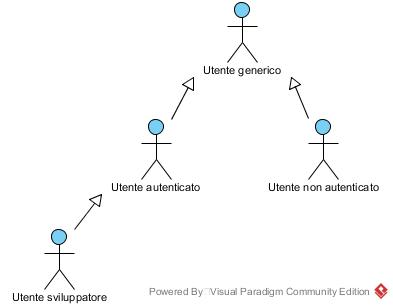
\includegraphics[width=9.7cm]{res/img/gerarchiaAttoriPrimari.jpg}
	\caption{Gerarchia attori primari}
\end{figure}

Sono state identificate quattro diverse tipologie di attori primari relazionati tra loro in maniera gerarchica:

\begin{itemize}
	\item \textbf{Utente generico:} utente che ha eseguito il comando per l'avvio dell'applicativo tramite \textit{Etherlesss-cli};
	\item \textbf{Utente non autenticato:} utente che non ha ancora eseguito l'accesso o la registrazione al network \textit{Ethereum\glo} e che dunque non potrà usufruire delle funzionalità dell'applicazione;
	\item \textbf{Utente autenticato:} utente che ha eseguito l'accesso al network \textit{Ethereum\glo} e che potrà eseguire i comandi messi a disposizione del servizio per gli utenti utilizzatori;
	\item \textbf{Utente sviluppatore:} utente che ha la possibilità di eseguire il \textit{deploy\glo} di funzioni JavaScript proprie, oltre che eseguire le altre funzioni messe a disposizione dagli altri utenti del servizio.
\end{itemize}


\subsubsection{Attori secondari}
Dall'analisi sui requisiti del sistema è emersa la presenza di un unico attore secondario:
\begin{itemize}
	\item \textbf{Ethereum\glo Network:} l'autenticazione a \textit{Etherless} coinciderà con l'accesso alla rete \textit{Ethereum\glos}. Oltre a ciò, l'\textit{Ethereum\glo} Network sarà coinvolto nei pagamenti tra gli utenti del sistema.
\end{itemize}


\newpage
\subsection{Elenco dei casi d'uso}

%\begin{figure}[h]
%	\centering
%	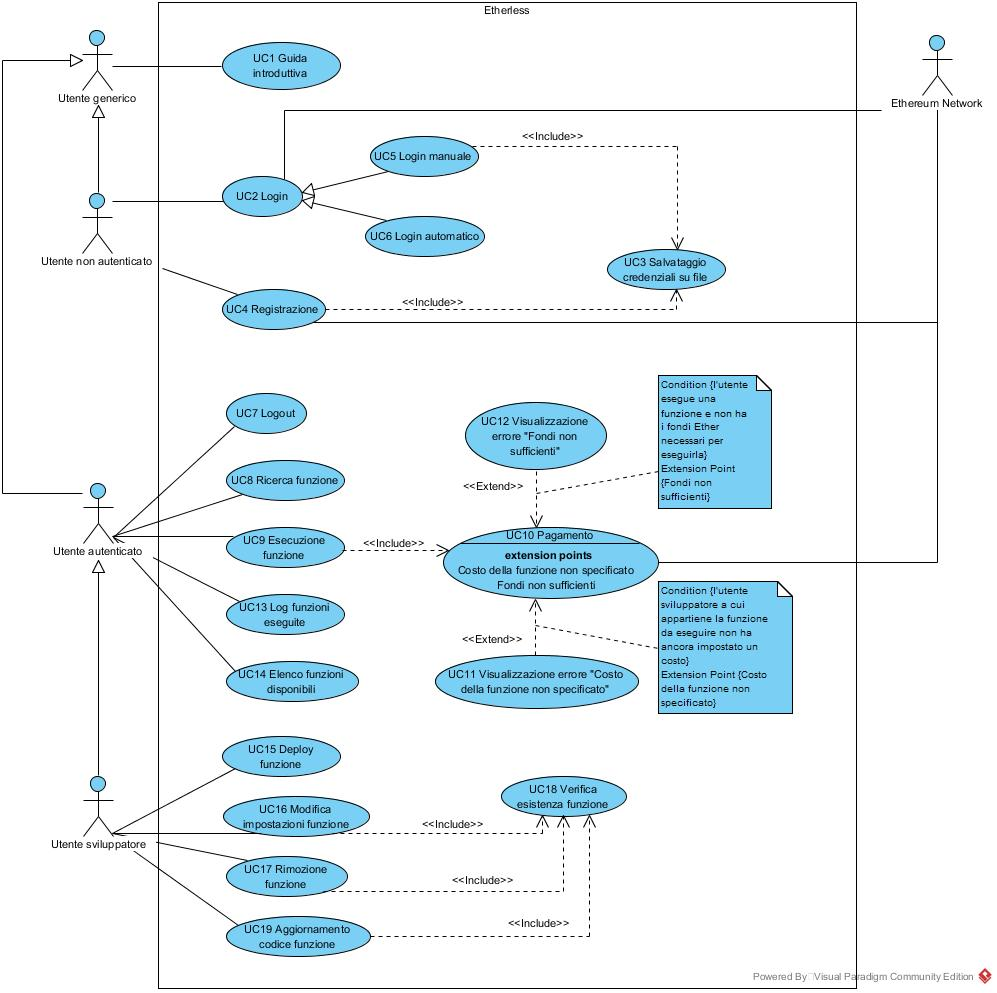
\includegraphics[width=12.3cm]{res/img/useCaseDiagram.jpg}
%	\caption{Casi d'uso principali}
%\end{figure}

\subsubsection{UC1 - Guida introduttiva}
\begin{itemize}
	\item \textbf{Attori primari:} Utente generico;
	\item \textbf{Descrizione:} l'utente generico, appena entrato nell'applicazione, visualizza una guida dei comandi utilizzabili; 
	\item \textbf{Pre-condizioni:} il sistema è raggiungibile e l'applicazione è stata avviata mediante l'apposito comando;
	\item \textbf{Post-condizioni:} Nella \textit{CLI\glo} vengono visualizzati i comandi utilizzabili dall'utente ed una loro descrizione;
	\item \textbf{Scenario principale:} L'utente visualizza la guida introduttiva.
\end{itemize}
\vspace{0.5cm}
\subsubsection{Visione ad alto livello - utente non autenticato}
\begin{figure}[h]
	\centering
	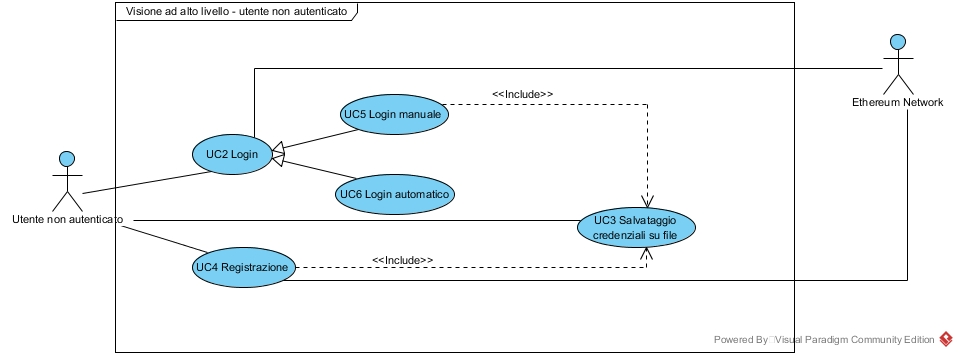
\includegraphics[width=\linewidth]{res/img/utenteNonAutenticato.jpg}
	\caption{Diagramma visione ad alto livello - utente non autenticato}
\end{figure}
\begin{itemize}
	\item \textbf{Attori primari:} Utente non autenticato;
	\item \textbf{Attori secondari:} \textit{Ethereum\glo} network;
	\item \textbf{Descrizione:} se l'utente non possiede una utenza \textit{Ethereum\glo} potrà registrarsi mediante la piattaforma oppure, in caso contrario, eseguire l'accesso con le proprie credenziali; 
	\item \textbf{Pre-condizioni:} l'utente ha avviato l'applicazione correttamente e ha visualizzato la guida introduttiva; 
	\item \textbf{Post-condizioni:} l'utente si sarà autenticato mediante registrazione o accesso a \textit{Eterium\glo} (con contestuale salvataggio delle credenziali su file) e potrà eseguire i comandi messi a disposizione dalla piattaforma;
	\item \textbf{Scenario principale:} 
	\begin{enumerate}
		\item L'utente può eseguire il login a \textit{Etherless} mediante utenza \textit{Ethereum\glo} (UC2);
		\item L'utente può eseguire il login manualmente inserendo le proprie credenziali tramite \textit{CLI\glo} (UC5);
		\item L'utente può eseguire il login automaticamente tramite le credenziali salvate su file (UC6);
		\item L'utente può eseguire la registrazione al network \textit{Etherium\glo} (UC4);
		\item Al primo accesso o alla registrazione al network \textit{Ethereum\glo} verranno automaticamente salvate le credenziali su file per facilitare accessi successivi (UC3).
	\end{enumerate}
\end{itemize}
\vspace{0.5cm}
\subsubsection{UC2 - Login}
\begin{itemize}
	\item \textbf{Attori primari:} Utente non autenticato;
	\item \textbf{Descrizione:} l'utente ha la possibilità di autenticarsi al network \textit{Ethereum\glo} mediante un address e di una \textit{private key\glos}; 
	\item \textbf{Pre-condizioni:} l'utente ha visualizzato la guida introduttiva e vuole eseguire l'accesso al network \textit{Ethereum};
	\item \textbf{Post-condizioni:} il sistema avrà autenticato o meno l'utente a seconda dei valori di accesso forniti;
	\item \textbf{Scenario principale:} 
	\begin{enumerate}
		\item Vengono inserite le credenziali di accesso (address e \textit{private key\glos}) in maniera manuale o automatica;
		\item L'utente viene autenticato al network \textit{Ethereum\glo} è può usufruire dei comandi messi a disposizione da \textit{Etherless}.
	\end{enumerate}
	\item \textbf{Specializzazioni:}
	\begin{itemize}
		\item \textbf{UC5:} l'utente ha la possibilità di eseguire il login manuale con l'inserimento di address e \textit{private key\glo} da \textit{CLI\glos};
		\item \textbf{UC6:} l'utente verrà automaticamente autenticato dal sistema se presente un file sul proprio dispositivo contenente le credenziali di accesso.  
	\end{itemize}
\end{itemize}
\vspace{0.5cm}
\subsubsection{UC5 - Login manuale}
\begin{figure}[h]
	\centering
	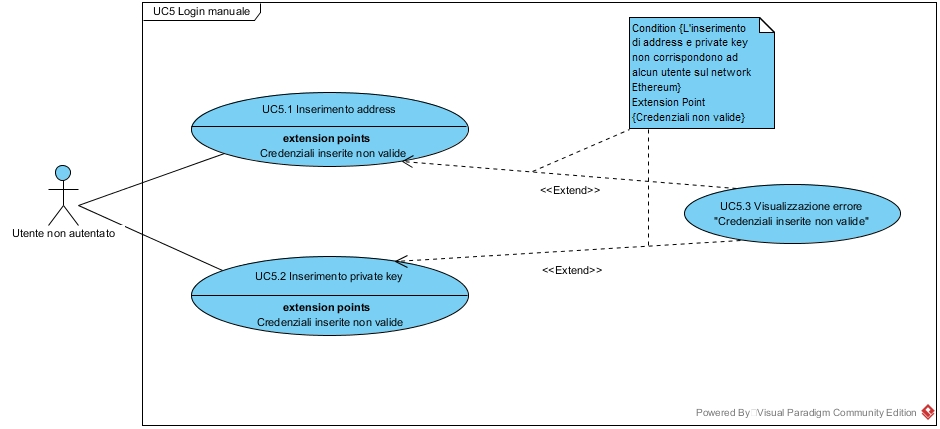
\includegraphics[width=0.8\linewidth]{res/img/UC5.jpg}
	\caption{Diagramma UC5 - Login manuale}
\end{figure}
\begin{itemize}
	\item \textbf{Attori primari:} Utente non autenticato;
	\item \textbf{Descrizione:} l'utente, mediante il comando "login" ha la possibilità di autenticarsi al network \textit{Ethereum\glo} inserendo manualmente da \textit{CLI\glo} il proprio address e \textit{private key\glos} e, contestualmente, salvare in automatico le credenziali di accesso su un file sul proprio dispositivo;
	\item \textbf{Pre-condizioni:} l'utente ha visualizzato la guida introduttiva e desidera autenticarsi manualmente;
	\item \textbf{Post-condizioni:} il sistema avrà autenticato o meno l'utente a seconda dei valori di accesso inseriti dalla \textit{CLI\glos};
	\item \textbf{Scenario principale:}
	\begin{enumerate}
		\item L'utente scriverà un comando da \textit{CLI\glos}, composto nel seguente modo:
		\begin{itemize}
			\item nome del comando "login";
			\item address;
			\item \textit{private key\glos};
			\item password
		\end{itemize}
		\item Verrà visualizzato a schermo un messaggio relativo all'esito dell'autenticazione;
		\item Sarà salvato un file sul dispositivo contenente le credenziali di accesso.
	\end{enumerate}
	\item \textbf{Estensioni:} 
	\begin{itemize}
		\item \textbf{UC5.3}: errore di autenticazione dovuto all'inserimento errato di address/\textit{private key\glos} non corrispondenti ad alcun account \textit{Ethereum\glos}.
	\end{itemize}
\end{itemize}

\vspace{0.5cm}
\subsubsection{UC5.1 - Inserimento address}
\begin{itemize}
	\item \textbf{Attori primari:} Utente non autenticato;
	\item \textbf{Descrizione:} l'utente potrà inserire tramite \textit{CLI\glo} l'address per l'autenticazione al suo account \textit{Ethereum\glos}; 
	\item \textbf{Pre-condizioni:} l'utente ha inserito il comando "login";
	\item \textbf{Post-condizioni:} l'utente ha inserito, a seguito del comando "login", il proprio address;
	\item \textbf{Scenario principale:} l'utente compila il comando per la richiesta di autenticazione inserendo il proprio address;
\end{itemize}
\vspace{0.5cm}
\subsubsection{UC5.2 - Inserimento private key\glo}
\begin{itemize}
	\item \textbf{Attori primari:} Utente non autenticato;
	\item \textbf{Descrizione:} l'utente potrà inserire tramite \textit{CLI\glo} la \textit{private key\glo} per l' autenticazione al suo account \textit{Ethereum\glos}; 
	\item \textbf{Pre-condizioni:} l'utente ha inserito il comando "login" seguito dal proprio address;
	\item \textbf{Post-condizioni:} l'utente ha inserito, a seguito dell'address, la propria \textit{private key\glos};
	\item \textbf{Scenario principale:} l'utente compila il comando per la richiesta di autenticazione inserendo la propria \textit{private key\glos};
	\item \textbf{Estensioni:} 
	\begin{itemize}
		\item \textbf{UC5.3}: errore di autenticazione dovuto all'inserimento errato di address e \textit{private key\glo} non corrispondenti ad alcun account \textit{Ethereum\glos}.
	\end{itemize}
\end{itemize}
\vspace{0.5cm}
\subsubsection{UC5.3 -Visualizzazione errore "Credenziali inserite non valide"}
\begin{itemize}
	\item \textbf{Attori primari:} Utente non autenticato;
    \item \textbf{Attori secondari:} \textit{Ethereum\glo} Network;
	\item \textbf{Descrizione:} il sistema, a seguito dell'inserimento delle credenziali per l'accesso ad \textit{Ethereum\glo} da parte dell'utente, restituisce un errore per il fallimento dell'autenticazione;
	\item \textbf{Pre-condizioni:} l'utente invia il comando "login" seguito da address e \textit{private key\glos};
	\item \textbf{Post-condizioni:} il sistema restituisce un errore sulla \textit{CLI\glo} in seguito al fallimento dell'autenticazione;
	\item \textbf{Scenario principale:} Il sistema notifica all'utente un errore avvenuto nella autenticazione al sistema tramite i valori da lui inseriti non corrispondenti ad alcuna utenza esistente. L'utente non sarà dunque autenticato al sistema e non potrà eseguire le funzionalità messe a disposizione da \textit{Etherless}.
\end{itemize}

\vspace{0.5cm}
\subsubsection{UC6 - Login Automatico}
\begin{itemize}
	\item \textbf{Attori primari:} Utente non autenticato;
	\item \textbf{Descrizione:} l'utente, se avrà già effettuato almeno una volta l'accesso alla rete \textit{Ethereum\glo} mediante l'applicazione \textit{Etherless}, potrà accedere automaticamente senza l'inserimento manuale delle credenziali; 
	\item \textbf{Pre-condizioni:} l'utente si è registrato oppure ha eseguito l'accesso almeno una volta mediante \textit{Ethereum};
	\item \textbf{Post-condizioni:} il sistema autenticherà l'utente a seconda dei valori di accesso inseriti nel file;
	\item \textbf{Scenario principale:} se il file è presente nel proprio dispositivo, l'utente avrà la possibilità di utilizzare tutti i comandi disponibili poichè automaticamente autenticato dal sistema. In caso il file risulti assente o corrotto, verrà richiesto il login manuale.
\end{itemize}
\vspace{0.5cm}
\subsubsection{UC4 - Registrazione}
\begin{figure}[h]
	\centering
	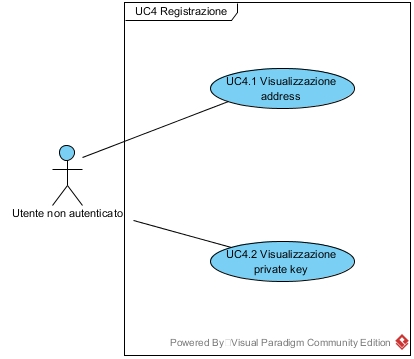
\includegraphics[width=0.7\linewidth]{res/img/UC4.jpg}
	\caption{Diagramma UC4 - Registrazione}
\end{figure}
\begin{itemize}
	\item \textbf{Attori primari:} Utente non autenticato;
	\item \textbf{Attori secondari:} \textit{Ethereum\glo} Network;
	\item \textbf{Descrizione:} l'utente, se non possiede un account \textit{Ethereum\glos}, potrà richiederne uno mediante il comando "signup"; 
	\item \textbf{Pre-condizioni:} l'utente ha visualizzato la guida introduttiva e vuole eseguire la registrazione al network \textit{Ethereum\glos};
	\item \textbf{Post-condizioni:} il sistema registrerà l'utente al network \textit{Ethereum\glo} e lo autenticherà al sistema;
	\item \textbf{Scenario principale:} 
	\begin{enumerate}
		\item L'utente inserisce il comando "signup" per la registrazione;
		\item Il sistema registrerà l'utenza sulla rete \textit{Ethereum\glos};
		\item L'utente risulterà autenticato al sistema;
		\item L'utente potrà vedere le proprie credenziali sulla \textit{CLI\glos};
		\item Sarà salvato un file sul dispositivo contenente le credenziali di accesso.
	\end{enumerate} 
\end{itemize}
\vspace{0.5cm}
\subsubsection{UC4.1 - Visualizzazione dati di registrazione}
\begin{itemize}
	\item \textbf{Attori primari:} Utente non autenticato;
	\item \textbf{Descrizione:} il sistema ha registrato correttamente l'utenza sul network \textit{Ethereum\glos} e stampa sulla CLI\glo  le credenziali di accesso generate casualmente dal Network; 
	\item \textbf{Pre-condizioni:} l'utente richiede un account \textit{Ethereum\glo} mediante il comando "signup"; 
	\item \textbf{Post-condizioni:} l'utente visualizzerà a schermo le proprie credenziali di accesso generate automaticamente dal network \textit{Ethereum\glos};
	\item \textbf{Scenario principale:} l'utente, dopo aver inserito il comando per la registrazione al network \textit{Ethereum\glo} visualizzerà sulla CLI il proprio address e la propria \textit{private-key\glo} generate automaticamente dal Network \textit{Ethereum\glos}.
\end{itemize}
\vspace{0.5cm}
\subsubsection{UC4.2 - Visualizzazione private key\glo}
\begin{itemize}
	\item \textbf{Attori primari:} Utente non autenticato;
	\item \textbf{Descrizione:} il sistema ha registrato correttamente l'utenza sul network \textit{Ethereum\glos} e stampa sulla CLI\glo la \textit{private key\glo} generata; 
	\item \textbf{Pre-condizioni:} l'utente richiede un account \textit{Ethereum\glo} mediante il comando "signup"; 
	\item \textbf{Post-condizioni:} l'utente visualizzerà a schermo la propria \textit{private key\glo} generata dal network \textit{Ethereum\glos};
	\item \textbf{Scenario principale:} l'utente, dopo aver inserito il comando per la registrazione al network \textit{Ethereum\glo} visualizzerà sulla CLI la propria \textit{private key\glo} generata automaticamente dal sistema.
\end{itemize}
\vspace{0.5cm}
\subsubsection{UC3 - Salvataggio su file}
\begin{itemize}
	\item \textbf{Attori primari:} Utente non autenticato;
	\item \textbf{Descrizione:} quando l'utente compierà per la prima volta l'accesso o si registrerà al network \textit{Ethereum\glo} mediante il sistema, verrà salvato un file sul suo dispositivo contenente le credenziali di accesso utili per i successivi login automatici; 
	\item \textbf{Pre-condizioni:} l'utente si sta autenticando mediante l'apposito comando al network \textit{Ethereum\glos};
	\item \textbf{Post-condizioni:} il sistema avrà salvato un file contenente address e \textit{private key\glo} sul dispositivo;
	\item \textbf{Scenario principale:} 
	\begin{enumerate}
		\item L'utente esegue l'autenticazione manuale o la registrazione mediante i comandi "login"o "signup";
		\item Il sistema salverà le credenziali per i futuri login automatici.
	\end{enumerate}
\end{itemize}
\vspace{0.5cm}

\newpage
\subsubsection{Visione ad alto livello - utente autenticato}
\begin{figure}[h]
	\centering
	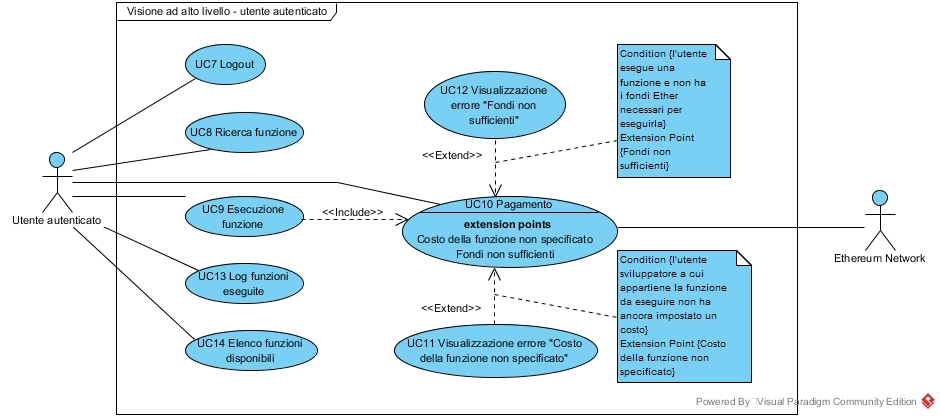
\includegraphics[width=\linewidth]{res/img/utenteAutenticato.jpg}
	\caption{Diagramma visione ad alto livello - utente autenticato}
\end{figure}
\begin{itemize}
	\item \textbf{Attori primari:} Utente autenticato;
	\item \textbf{Attori secondari:} \textit{Ethereum\glo} network;
	\item \textbf{Descrizione:} l'utente che ha eseguito l'autenticazione a \textit{Etherless} mediante l'utenza \textit{Ethereum\glo} potrà eseguire i comandi relativi ad un utente utilizzatore; 
	\item \textbf{Pre-condizioni:} l'utente ha eseguito l'accesso al sistema; 
	\item \textbf{Post-condizioni:} l'utente potrà eseguire i comandi messi a disposizione per gli utenti utilizzatori della piattaforma;
	\item \textbf{Scenario principale:} 
	\begin{enumerate}
		\item L'utente può eseguire il logout da \textit{Etherless} (UC7);
		\item L'utente può cercare i dettagli di una funzione presente nel sistema (UC8);
		\item L'utente può eseguire una funzione presente nel sistema (UC9);
		\item L'utente può pagare allo sviluppatore della funzione e ai gestori del servizio una somma in \textit{Ether\glo} per aver eseguito una determinata funzione (UC10);
		\item L'utente può visualizzare errori relativi al pagamento per "fondi non sufficienti" (UC12);
		\item L'utente può visualizzare errori relativi al pagamento per "costo della funzione non specificato" (UC11);
		\item L'utente può eseguire il log delle funzioni da lui eseguite (UC13);
		\item L'utente può visualizzare l'elenco delle funzioni disponibili nel sistema (UC14).
	\end{enumerate}
\end{itemize}
\subsubsection{UC7 - Logout}
\begin{itemize}
	\item \textbf{Attori primari:} Utente autenticato;
	\item \textbf{Descrizione:} l'utente autenticato vuole eseguire il logout dal sistema eliminando il file contenente le credenziali di accesso; 
	\item \textbf{Pre-condizioni:} l'utente ha effettuato l'accesso ad \textit{Etherless};
	\item \textbf{Post-condizioni:} verrà eseguito il logout dell'utente autenticato;
	\item \textbf{Scenario principale:} 
	\begin{itemize}
		\item L'utente inserisce il comando per il logout;
		\item Il sistema eseguirà il logout dell'utenza sulla rete \textit{Ethereum\glos} e cancellerà il file di accesso.
	\end{itemize}
\end{itemize}
\vspace{0.5cm}
\subsubsection{UC7 - Ricerca funzione}

\vspace{0.5cm}
\subsubsection{UC8.1 - Inserimento nome funzione da cercare}
\begin{itemize}
	\item \textbf{Attori primari:} Utente autenticato;
	\item \textbf{Descrizione:} l'utente potrà inserire tramite \textit{CLI} il nome della funzione presente su \textit{Etherless} della quale vedere i dettagli; 
	\item \textbf{Pre-condizioni:} l'utente ha inserito il comando "find";
	\item \textbf{Post-condizioni:} l'utente ha inserito, a seguito del comando "find", il nome della funzione da cercare;
	\item \textbf{Scenario principale:} l'utente inserisce il nome della funzione di cui visualizzare i dettagli;
	\item \textbf{Estensioni:} 
	\begin{itemize}
		\item \textbf{UC8.2}: se non è presente in \textit{Etherless} alcuna funzione con il nome inserito, verrà visualizzato un messaggio di errore.
	\end{itemize}
\end{itemize}
\vspace{0.5cm}
\subsubsection{UC8.2 - Visualizzazione risultati ricerca}
\begin{itemize}
	\item \textbf{Attori primari:} Utente autenticato;
	\item \textbf{Descrizione:} l'utente visualizzerà sul \textit{CLI\glo} il risultato della ricerca della funzione della quale potrà vedere i dettagli;
	\item \textbf{Pre-condizioni:} l'utente ha eseguito il comando "find";
	\item \textbf{Post-condizioni:} \textit{CLI\glo} visualizza il risultato;
	\item \textbf{Scenario principale:} Il sistema mostrerà sulla \textit{CLI\glo} le seguenti informazioni della funzione:
    		\begin{itemize}
    			\item autore;
    			\item costo;
    			\item descrizione;
    			\item firma della funzione.
    		\end{itemize}
\end{itemize}

\vspace{0.5cm}
\subsubsection{UC8.2.1 - Visualizzazione autore funzione}
\begin{itemize}
	\item \textbf{Attori primari:} Utente autenticato;
	\item \textbf{Descrizione:} l'utente ha eseguito con successo la ricerca della funzione e ne visualizza le informazioni a riguardo. In particolar modo ne verrà visualizzato l'autore; 
	\item \textbf{Pre-condizioni:} l'utente richiede le informazioni di una funzione presente su \textit{Etherless} mediante il comando "find"; 
	\item \textbf{Post-condizioni:} l'utente visualizzerà a schermo l'autore della funzione scelta;
	\item \textbf{Scenario principale:} l'utente, dopo aver inserito il comando per la ricerca di una funzione, visualizzerà sulla \textit{CLI\glo} l'autore della stessa.
\end{itemize}
\vspace{0.5cm}
\subsubsection{UC8.2.2 - Visualizzazione costo funzione}
\begin{itemize}
	\item \textbf{Attori primari:} Utente autenticato;
	\item \textbf{Descrizione:} l'utente ha eseguito con successo la ricerca della funzione e ne visualizza le informazioni a riguardo. In particolar modo ne verrà visualizzato il costo; 
	\item \textbf{Pre-condizioni:} l'utente richiede le informazioni di una funzione presente su \textit{Etherless} mediante il comando "find"; 
	\item \textbf{Post-condizioni:} l'utente visualizzerà a schermo il costo della funzione scelta;
	\item \textbf{Scenario principale:} l'utente, dopo aver inserito il comando per la ricerca di una funzione, visualizzerà sulla \textit{CLI\glo} il costo della stessa.
\end{itemize}
\vspace{0.5cm}
\subsubsection{UC8.2.3 - Visualizzazione descrizione funzione}
\begin{itemize}
	\item \textbf{Attori primari:} Utente autenticato;
	\item \textbf{Descrizione:} l'utente ha eseguito con successo la ricerca della funzione e ne visualizza le informazioni a riguardo. In particolar modo ne verrà visualizzata la descrizione; 
	\item \textbf{Pre-condizioni:} l'utente richiede le informazioni di una funzione presente su \textit{Etherless} mediante il comando "find"; 
	\item \textbf{Post-condizioni:} l'utente visualizzerà a schermo la descrizione della funzione scelta;
	\item \textbf{Scenario principale:} l'utente, dopo aver inserito il comando per la ricerca di una funzione, visualizzerà sulla \textit{CLI\glo} la descrizione della stessa.
\end{itemize}
\vspace{0.5cm}
\subsubsection{UC8.2.4 - Visualizzazione firma funzione}
\begin{itemize}
	\item \textbf{Attori primari:} Utente autenticato;
	\item \textbf{Descrizione:} l'utente ha eseguito con successo la ricerca della funzione e ne visualizza le informazioni a riguardo. In particolar modo ne verrà visualizzata la firma; 
	\item \textbf{Pre-condizioni:} l'utente richiede le informazioni di una funzione presente su \textit{Etherless} mediante il comando "find"; 
	\item \textbf{Post-condizioni:} l'utente visualizzerà a schermo la firma della funzione scelta;
	\item \textbf{Scenario principale:} l'utente, dopo aver inserito il comando per la ricerca di una funzione, visualizzerà sulla \textit{CLI\glo} la firma della stessa.
\end{itemize}
\vspace{0.5cm}
\subsubsection{UC8.3 - Visualizzazione errore "Funzione non esistente"}
\begin{itemize}
	\item \textbf{Attori primari:} Utente autenticato;
	\item \textbf{Descrizione:} il sistema, a seguito dell'inserimento di un nome di funzione non esistente su \textit{Etherless} e all'invio del comando, restituirà un errore;
	\item \textbf{Pre-condizioni:} l'utente invia il comando "find" seguito dal nome della funzione da ricercare;
	\item \textbf{Post-condizioni:} il sistema restituisce un errore sulla \textit{CLI\glo} dopo non aver trovato la funzione richiesta tra le disponibili;
	\item \textbf{Scenario principale:} il sistema notifica all'utente l'assenza della funzione ricercata.
\end{itemize}

\vspace{0.5cm}
\subsubsection{UC9 - Ricerca funzione}
\begin{figure}[h]
	\centering
	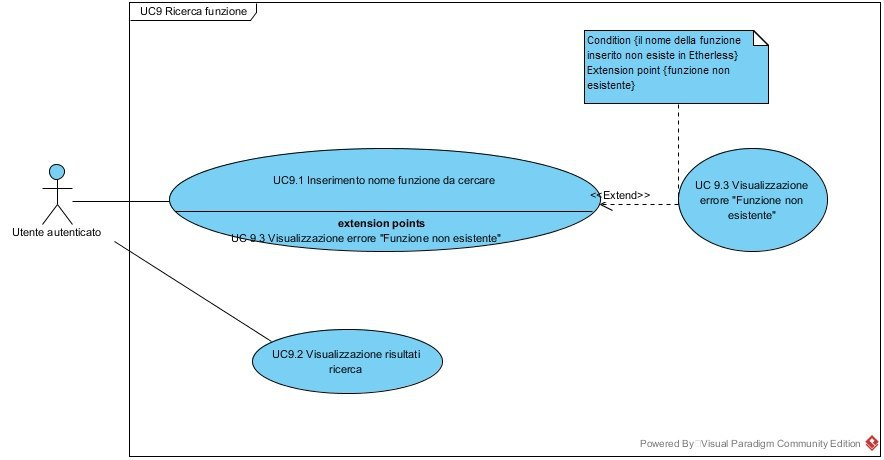
\includegraphics[width=\linewidth]{res/img/UC9.jpg}
	\caption{Diagramma UC9 - Ricerca funzione}
\end{figure}
\begin{itemize}
	\item \textbf{Attori primari:} Utente autenticato;
	\item \textbf{Descrizione:} l'utente autenticato ricerca per nome i dettagli di una specifica funzione caricata da un utente sviluppatore sulla rete \textit{Etherless};
	\item \textbf{Pre-condizioni:} l'utente ha effettuato l'accesso ad \textit{Etherless} e vuole ricercare una funzione specifica mediante l'apposito comando;
	\item \textbf{Post-condizioni:} il sistema visualizzerà a schermo i dettagli della funzione ricercata o un messaggio di errore se la funzione non è stata trovata;
	\item \textbf{Scenario principale:}
	\begin{enumerate}
		\item L'utente scriverà un comando da \textit{CLI\glos} composto nel seguente modo:
		\begin{itemize}
			\item nome del comando "find";
			\item nome della funzione da ricercare.
		\end{itemize}
        \item L'utente visualizzerà la funzione ricercata e i suoi dettagli.
	\end{enumerate}
\end{itemize}

\vspace{0.5cm}
\subsubsection{UC9.1 - Inserimento nome funzione da cercare}
\begin{itemize}
	\item \textbf{Attori primari:} Utente autenticato;
	\item \textbf{Descrizione:} l'utente potrà inserire tramite \textit{CLI\glo} il nome della funzione presente su \textit{Etherless};
	\item \textbf{Pre-condizioni:} l'utente ha inserito il comando "find";
	\item \textbf{Post-condizioni:} l'utente ha inserito, a seguito del comando "find", il nome della funzione da cercare;
	\item \textbf{Scenario principale:} l'utente inserisce il nome della funzione di cui visualizzare i dettagli;
	\item \textbf{Estensioni:}
	\begin{itemize}
		\item \textbf{UC9.2}: l'inserimento del comando find provoca la visualizzazione dei risultati;
		\item \textbf{UC9.3}: se non è presente in \textit{Etherless} alcuna funzione con il nome inserito, verrà visualizzato un messaggio di errore.
	\end{itemize}
\end{itemize}

\vspace{0.5cm}
\subsubsection{UC9.2 - Inserimento parametri funzione}
\begin{itemize}
	\item \textbf{Attori primari:} Utente autenticato;
	\item \textbf{Descrizione:} l'utente potrà inserire tramite \textit{CLI\glos}il valore dei parametri della funzione presente su \textit{Etherless} da eseguire; 
	\item \textbf{Pre-condizioni:} l'utente ha inserito da \textit{CLI\glo} il comando "run" seguito dal nome della funzione di interesse;
	\item \textbf{Post-condizioni:} l'utente ha inserito, a seguito del nome della funzione da eseguire, i valori dei parametri;
	\item \textbf{Scenario principale:} l'utente inserisce i valori dei parametri della funzione che vuole eseguire;
	\item \textbf{Estensioni:} 
	\begin{itemize}
		\item \textbf{UC9.4}: se il numero dei parametri inseriti non corrispondono ai parametri richiesti dalla funzione inserita.
	\end{itemize}
\end{itemize}
\vspace{0.5cm}
\subsubsection{UC9.3 - Visualizzazione errore "Funzione non esistente"}
\begin{itemize}
	\item \textbf{Attori primari:} Utente autenticato;
	\item \textbf{Descrizione:} il sistema, a seguito dell'inserimento di un nome di funzione non esistente su \textit{Etherless} e all'invio del comando, restituirà un errore;
	\item \textbf{Pre-condizioni:} l'utente invia il comando "find" seguito dal nome della funzione da ricercare;
	\item \textbf{Post-condizioni:} il sistema restituisce un errore sulla \textit{CLI\glo} dopo non aver trovato la funzione richiesta tra le disponibili;
	\item \textbf{Scenario principale:} il sistema notifica all'utente l'assenza della funzione ricercata.
\end{itemize}

\vspace{0.5cm}
\subsubsection{UC9.4 - Visualizzazione errore "Numero dei parametri non corrispondente"}
\begin{itemize}
	\item \textbf{Attori primari:} Utente autenticato;
	\item \textbf{Descrizione:} il sistema, a seguito dell'inserimento di un numero errato di parametri e dell'invio del comando, restituirà un errore; 
	\item \textbf{Pre-condizioni:} l'utente invia il comando "run" seguito dal nome della funzione da ricercare e i valori dei parametri;
	\item \textbf{Post-condizioni:} il sistema restituisce un errore sulla \textit{CLI\glo} dopo non aver trovato corrispondenza tra numero dei parametri richiesti dalla funzione e i valori inseriti dall'utente;
	\item \textbf{Scenario principale:} il sistema notifica all'utente la non corrispondenza del numero dei parametri inseriti con quelli richiesti dalla funzione specificata nel comando;
\end{itemize}


\vspace{0.5cm}
\subsubsection{UC10 - Esecuzione funzione}
\begin{figure}[h]
	\centering
	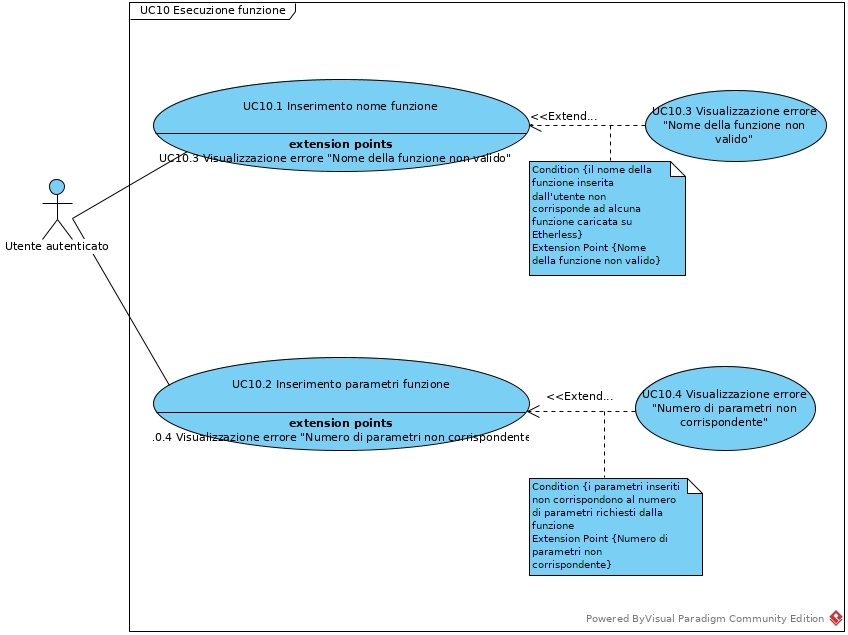
\includegraphics[width=\linewidth]{res/img/UC10.jpg}
	\caption{Diagramma UC10 - Esecuzione funzione}
\end{figure}
\begin{itemize}
	\item \textbf{Attori primari:} Utente autenticato;
	\item \textbf{Descrizione:} l'utente autenticato esegue una delle funzioni disponibili sulla piattaforma \textit{Etherless} tramite il comando "run";
	\item \textbf{Pre-condizioni:} l'utente ha effettuato l'accesso ad \textit{Etherless} e vuole eseguire una tra le funzioni messe a disposizione dagli utenti sviluppatori pagando la somma richiesta;
	\item \textbf{Post-condizioni:} il sistema visualizzerà a schermo l'output della funzione eseguita dall'utente;
	\item \textbf{Scenario principale:}
	\begin{enumerate}
		\item L'utente scriverà un comando da \textit{CLI\glo} composto nel seguente modo:
		\begin{itemize}
			\item nome del comando "run";
			\item nome della funzione;
			\item valore dei parametri.
			\item password per accedere alle credenziali salvate in locale e firmare l'avvenuta transazione.
		\end{itemize}
		\item Se il sistema non rileva errori durante dopo l'invio del comando, viene eseguito il pagamento per l'esecuzione della funzione;
		\item Il sistema, dopo aver eseguito la funzione richiesta, mostrerà sulla \textit{CLI\glo} l'output in base al valore dei parametri inseriti;
		\item Al termine viene salvato in un file locale, apposito, il log. Il file viene creato in automatico alla prima richiesta di esecuzione.
	\end{enumerate}
	\item \textbf{Inclusioni:}
	\begin{itemize}
		\item \textbf{UC11:} Ogni qualvolta l'utente esegua una funzione, deve necessariamente corrispondere il pagamento della cifra imposta dall'utente sviluppatore.
	\end{itemize}
\end{itemize}

\vspace{0.5cm}
\subsubsection{UC11 - Visualizzazione errore "Costo della funzione non specificato"}
\begin{itemize}
	\item \textbf{Attori primari:} Utente autenticato;
	\item \textbf{Descrizione:} il sistema, in seguito al tentativo di esecuzione e pagamento di una delle funzioni disponibili da parte di un utente, gli notifica che il costo della stessa non è ancora stato impostato dallo sviluppatore; 
	\item \textbf{Pre-condizioni:} l'utente ha utilizzato il comando "run" per l'esecuzione di una specifica funzione;
	\item \textbf{Post-condizioni:} il sistema notifica un messaggio di errore riguardo l'assenza del costo di esecuzione della funzione;
	\item \textbf{Scenario principale:} 
	\begin{enumerate}
		\item L'utente tenta l'esecuzione di una funzione utilizzando il comando "run";
		\item Il sistema interrompe l'esecuzione notificando all'utente che non è stato specificato alcun costo per l'esecuzione della funzione.
	\end{enumerate}
\end{itemize}
\vspace{0.5cm}
\subsubsection{UC12 - Visualizzazione errore "Fondi non sufficienti"}
\begin{itemize}
	\item \textbf{Attori primari:} Utente autenticato;
	\item \textbf{Descrizione:} il sistema, in seguito al tentativo di esecuzione e pagamento di una delle funzioni disponibili da parte di un utente, gli notifica che non dispone di crediti \textit{Ether\glo} a sufficienza; 
	\item \textbf{Pre-condizioni:} l'utente ha utilizzato il comando "run" per l'esecuzione di una specifica funzione;
	\item \textbf{Post-condizioni:} il sistema notifica un messaggio di errore riguardo l'assenza di crediti \textit{Ether\glos};
	\item \textbf{Scenario principale:} 
	\begin{enumerate}
		\item L'utente tenta l'esecuzione di una funzione con il comando "run";
		\item Il sistema interrompe l'esecuzione notificando all'utente che l'importo da corrispondere supera i crediti \textit{Ether\glo} presenti nel suo wallet.
	\end{enumerate}
\end{itemize}
\vspace{0.5cm}
\subsubsection{UC13 - Log funzioni eseguite}
\begin{itemize}
	\item \textbf{Attori primari:} Utente autenticato;
	\item \textbf{Descrizione:} l'utente visualizza il log delle funzioni da lui eseguite mediante l'apposito comando; 
	\item \textbf{Pre-condizioni:} l'utente ha utilizzato il comando per la visualizzazione del log;
	\item \textbf{Post-condizioni:} il sistema visualizzerà sulla \textit{CLI\glo} il log delle funzioni eseguite dall'utente;
	\item \textbf{Scenario principale:} 
	\begin{enumerate}
		\item L'utente richiede il log mediante l'apposito comando;
		\item Il sistema visualizzerà su schermo i log con le seguenti informazioni:
		\begin{itemize}
			\item data e ora di esecuzione della funzione;
			\item nome della funzione eseguita
			\item firma della funzione;
			\item costo della funzione.
		\end{itemize}
	\end{enumerate}
\end{itemize}
\vspace{0.5cm}
\subsubsection{UC13.1 - Visualizzazione funzioni log}
\begin{itemize}
	\item \textbf{Attori primari:} Utente autenticato;
	\item \textbf{Descrizione:} l'utente visualizza il log delle funzioni da lui eseguite mediante l'apposito comando "log"; 
	\item \textbf{Pre-condizioni:} l'utente ha utilizzato il comando per la visualizzazione del log;
	\item \textbf{Post-condizioni:} il sistema visualizzerà sulla \textit{CLI\glo} il log delle funzioni eseguite dall'utente;
	\item \textbf{Scenario principale:} 
	\begin{enumerate}
		\item L'utente richiede il log mediante il comando "log";
		\item Il sistema visualizzerà su schermo i log con le seguenti informazioni:
		\begin{itemize}
			\item data e ora di esecuzione della funzione;
			\item nome della funzione eseguita;
			\item firma della funzione;
			\item costo della funzione.
		\end{itemize}
	\end{enumerate}
\end{itemize}
\vspace{0.5cm}
\subsubsection{UC13.2 - Visualizzazione del log delle funzioni eseguite}
\begin{figure}[h]
	\centering
	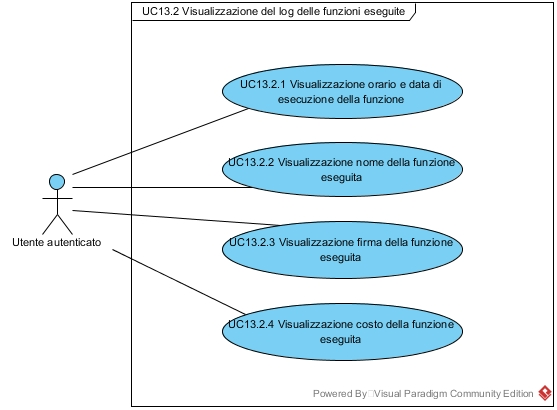
\includegraphics[width=0.7\linewidth]{res/img/UC13.2.jpg}
	\caption{Diagramma UC13.2 - Visualizzazione del log delle funzioni eseguite"}
\end{figure}
\begin{itemize}
	\item \textbf{Attori primari:} Utente autenticato;
	\item \textbf{Descrizione:} l'utente visualizzerà sul \textit{CLI\glo} il risultato del comando "log";
	\item \textbf{Pre-condizioni:} l'utente ha eseguito il comando "log";
	\item \textbf{Post-condizioni:} \textit{CLI\glo} il log relativo alle funzioni da lui eseguite;
	\item \textbf{Scenario principale:} Il sistema mostrerà sulla \textit{CLI\glo} le informazioni relative a tutte le esecuzioni delle funzioni effettuate dall'utente.
\end{itemize}
\vspace{0.5cm}
\subsubsection{UC13.2.1 - Visualizzazione della funzione in log}
\begin{figure}[h]
	\centering
	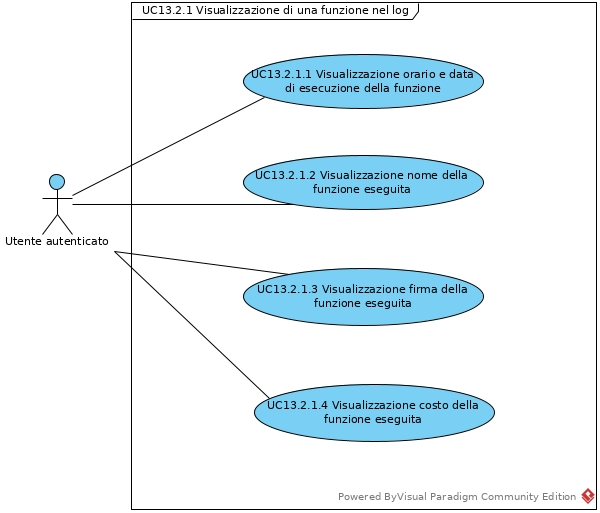
\includegraphics[width=0.7\linewidth]{res/img/UC13.2.1.jpg}
	\caption{Diagramma UC13.2.1 - Visualizzazione della funzione in log"}
\end{figure}
\begin{itemize}
	\item \textbf{Attori primari:} Utente autenticato;
	\item \textbf{Descrizione:} l'utente visualizzerà sul \textit{CLI\glo} i dettagli di una singola funzione;
	\item \textbf{Pre-condizioni:} l'utente ha eseguito il comando "log" e ha visualizzato il log delle funzioni;
	\item \textbf{Post-condizioni:} dettagli di una singola funzione;
	\item \textbf{Scenario principale:} Il sistema mostrerà sulla \textit{CLI\glo} le informazioni relative a una singola funzione.
\end{itemize}

\vspace{0.5cm}
\subsubsection{UC13.2.2 - Visualizzazione nome della funzione eseguita}
\begin{itemize}
	\item \textbf{Attori primari:} Utente autenticato;
	\item \textbf{Descrizione:} l'utente ha eseguito con successo il comando "log" e visualizza le informazioni relative alle ultime funzioni da lui eseguite. In particolare verrà visualizzato, per ciascuna di esse, il nome; 
	\item \textbf{Pre-condizioni:} l'utente richiede il log delle funzioni da lui eseguite mediante il comando "log"; 
	\item \textbf{Post-condizioni:} l'utente visualizzerà a schermo il nome delle ultime funzioni eseguite;
	\item \textbf{Scenario principale:} l'utente, dopo aver inserito il comando per il log delle funzioni, visualizzerà sulla \textit{CLI\glo} il nome delle stesse.
\end{itemize}
\vspace{0.5cm}
\subsubsection{UC13.2.3 - Visualizzazione firma della funzione eseguita}
\begin{itemize}
	\item \textbf{Attori primari:} Utente autenticato;
	\item \textbf{Descrizione:} l'utente ha eseguito con successo il comando "log" e visualizza le informazioni relative alle ultime funzioni da lui eseguite. In particolare verrà visualizzato, per ciascuna di esse, la rispettiva firma; 
	\item \textbf{Pre-condizioni:} l'utente richiede il log delle funzioni da lui eseguite mediante il comando "log"; 
	\item \textbf{Post-condizioni:} l'utente visualizzerà a schermo la firma delle ultime funzioni eseguite;
	\item \textbf{Scenario principale:} l'utente, dopo aver inserito il comando per il log delle funzioni, visualizzerà sulla \textit{CLI\glo} la firma delle stesse.
\end{itemize}
\vspace{0.5cm}
\subsubsection{UC13.2.4 - Visualizzazione costo della funzione eseguita}
\begin{itemize}
	\item \textbf{Attori primari:} Utente autenticato;
	\item \textbf{Descrizione:} l'utente ha eseguito con successo il comando "log" e visualizza le informazioni relative alle ultime funzioni da lui eseguite. In particolare verrà visualizzato, per ciascuna di esse, il costo; 
	\item \textbf{Pre-condizioni:} l'utente richiede il log delle funzioni da lui eseguite mediante il comando "log"; 
	\item \textbf{Post-condizioni:} l'utente visualizzerà a schermo il costo delle ultime funzioni eseguite;
	\item \textbf{Scenario principale:} l'utente, dopo aver inserito il comando per il log delle funzioni, visualizzerà sulla \textit{CLI\glo} il costo delle stesse.
\end{itemize}
\vspace{0.5cm}
\subsubsection{UC13.3 - Log funzioni vuoto}
\begin{itemize}
	\item \textbf{Attori primari:} Utente autenticato;
	\item \textbf{Descrizione:} l'utente visualizza il log delle funzioni da lui eseguite mediante l'apposito comando "log"; 
	\item \textbf{Pre-condizioni:} l'utente ha utilizzato il comando per la visualizzazione del log;
	\item \textbf{Post-condizioni:} il sistema visualizzerà sulla \textit{CLI\glo} un messaggio di errore per log assente;
	\item \textbf{Scenario principale:} 
	\begin{enumerate}
		\item L'utente richiede il log mediante il comando "log";
		\item Il sistema visualizzerà su schermo un messaggio contente "Log funzioni vuoto".
	\end{enumerate}
\end{itemize}
\vspace{0.5cm}
\subsubsection{UC14 - Log funzioni eseguite}
\begin{figure}[h]
	\centering
	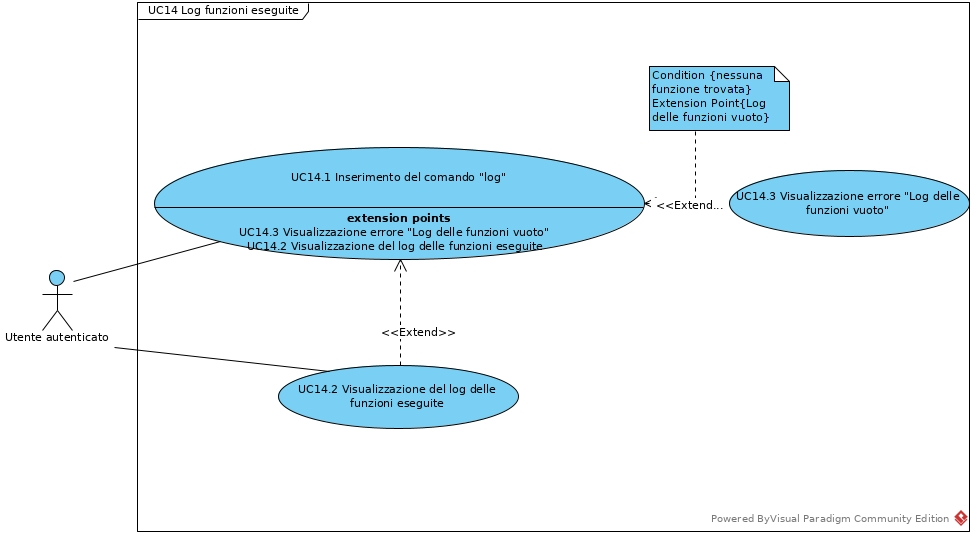
\includegraphics[width=\linewidth]{res/img/UC14.jpg}
	\caption{Diagramma UC14 - Log funzioni eseguite}
\end{figure}
\begin{itemize}
	\item \textbf{Attori primari:} Utente autenticato;
	\item \textbf{Descrizione:} l'utente prova a visualizzare il log delle funzioni da lui eseguite mediante l'apposito comando "log";
	\item \textbf{Pre-condizioni:} l'utente ha utilizzato il comando per la visualizzazione del log;
	\item \textbf{Post-condizioni:} il sistema visualizzerà sulla \textit{CLI\glo} il log delle funzioni eseguite dall'utente oppure visualizzerà sulla schermata "Log funzioni vuote";
	\item \textbf{Estensioni:}
	\begin{itemize}
		\item \textbf{UC14.3}: se l'utente non ha eseguito ancora alcuna funzione tra quelle presenti nel sistema \textit{Etherless\glos}, verrà restituito un messaggio di errore.
	\end{itemize}
\end{itemize}

\vspace{0.5cm}
\subsubsection{UC14.1 - Inserimento del comando "log"}
\begin{itemize}
	\item \textbf{Attori primari:} Utente autenticato;
	\item \textbf{Descrizione:} l'utente visualizza il log delle funzioni da lui eseguite mediante l'apposito comando "log"; 
	\item \textbf{Pre-condizioni:} l'utente ha utilizzato il comando per la visualizzazione del log;
	\item \textbf{Post-condizioni:} il sistema visualizzerà sulla \textit{CLI\glo} il log delle funzioni eseguite dall'utente;
	\item \textbf{Scenario principale:} 
	\begin{enumerate}
		\item L'utente richiede il log mediante il comando "log";
		\item Il sistema visualizzerà su schermo i log con le seguenti informazioni:
		\begin{itemize}
			\item data e ora di esecuzione della funzione;
			\item nome della funzione eseguita;
			\item firma della funzione;
			\item costo della funzione.
		\end{itemize}
	\end{enumerate}
	\item \textbf{Estensioni:}
	\begin{itemize}
		\item \textbf{UC14.3}: se l'utente non ha eseguito ancora alcuna funzione tra quelle presenti nel sistema \textit{Etherless\glos}, verrà restituito un messaggio di errore.
	\end{itemize}
\end{itemize}
\vspace{0.5cm}
\subsubsection{UC14.2 - Visualizzazione del log delle funzioni eseguite}
\begin{itemize}
	\item \textbf{Attori primari:} Utente autenticato;
	\item \textbf{Descrizione:} l'utente visualizzerà sul \textit{CLI\glo} il risultato del comando "log";
	\item \textbf{Pre-condizioni:} l'utente ha eseguito il comando "log";
	\item \textbf{Post-condizioni:} \textit{CLI\glo} il log relativo alle funzioni da lui eseguite;
	\item \textbf{Scenario principale:} Il sistema mostrerà sulla \textit{CLI\glo} le informazioni relative a tutte le esecuzioni delle funzioni effettuate dall'utente.
\end{itemize}

\vspace{0.5cm}
\subsubsection{UC14.2.1 Vis. log della funzione in lista}
\begin{figure}[h]
	\centering
	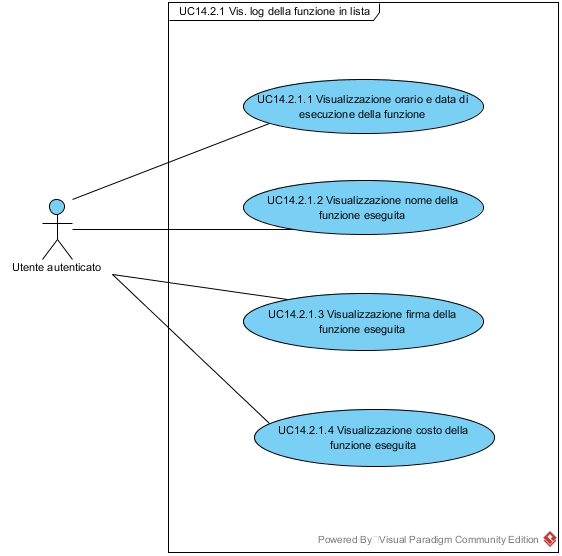
\includegraphics[width=0.7\linewidth]{res/img/UC14.2.1.jpg}
	\caption{Diagramma UC14.2.1 - Visualizzazione della singola funzione in "log"}
\end{figure}
\begin{itemize}
	\item \textbf{Attori primari:} Utente autenticato;
	\item \textbf{Descrizione:} l'utente visualizzerà sul \textit{CLI\glo} i dettagli di una singola funzione;
	\item \textbf{Pre-condizioni:} l'utente ha eseguito il comando "log" e ha visualizzato il log delle funzioni;
	\item \textbf{Post-condizioni:} dettagli di una singola funzione;
	\item \textbf{Scenario principale:} Il sistema mostrerà sulla \textit{CLI\glo} le informazioni relative a una singola funzione.
\end{itemize}

\vspace{0.5cm}
\subsubsection{UC14.2.2 - Visualizzazione costi delle funzioni disponibili}
\begin{itemize}
	\item \textbf{Attori primari:} Utente autenticato;
	\item \textbf{Descrizione:} l'utente ha eseguito con successo il comando "list" e visualizza le informazioni relative a ciascuna funzione presente su \textit{Etherless}. In particolar modo, per ciascuna di esse, verrà visualizzato il costo; 
	\item \textbf{Pre-condizioni:} l'utente richiede la lista delle funzioni presenti su \textit{Etherless} mediante il comando "list"; 
	\item \textbf{Post-condizioni:} l'utente visualizzerà a schermo il costo delle funzioni disponibili;
	\item \textbf{Scenario principale:} l'utente, dopo aver inserito il comando per la lista delle funzioni, visualizzerà sulla \textit{CLI\glo} i costi delle stesse.
\end{itemize}
\vspace{0.5cm}
\subsubsection{UC14.2.3 - Visualizzazione firme delle funzioni disponibili}
\begin{itemize}
	\item \textbf{Attori primari:} Utente autenticato;
	\item \textbf{Descrizione:} l'utente ha eseguito con successo il comando "list" e visualizza le informazioni relative a ciascuna funzione presente su \textit{Etherless}. In particolar modo, per ciascuna di esse, verranno visualizzate le relative firme; 
	\item \textbf{Pre-condizioni:} l'utente richiede la lista delle funzioni presenti su \textit{Etherless} mediante il comando "list"; 
	\item \textbf{Post-condizioni:} l'utente visualizzerà a schermo le firme delle funzioni disponibili;
	\item \textbf{Scenario principale:} l'utente, dopo aver inserito il comando per la lista delle funzioni, visualizzerà sulla \textit{CLI\glo} le firme delle stesse.
\end{itemize}
\vspace{0.5cm}
\subsubsection{UC14.2.4 - Visualizzazione descrizioni delle funzioni disponibili}
\begin{itemize}
	\item \textbf{Attori primari:} Utente autenticato;
	\item \textbf{Descrizione:} l'utente ha eseguito con successo il comando "list" e visualizza le informazioni relative a ciascuna funzione presente su \textit{Etherless}. In particolar modo, per ciascuna di esse, verrà visualizzata la descrizione; 
	\item \textbf{Pre-condizioni:} l'utente richiede la lista delle funzioni presenti su \textit{Etherless} mediante il comando "list"; 
	\item \textbf{Post-condizioni:} l'utente visualizzerà a schermo la descrizione delle funzioni disponibili;
	\item \textbf{Scenario principale:} l'utente, dopo aver inserito il comando per la lista delle funzioni, visualizzerà sulla \textit{CLI\glo} le descrizioni delle stesse.
\end{itemize}
\vspace{0.5cm}
\subsubsection{UC14.3 - Visualizzazione errore "Nessuna funzione presente su Etherless\glos"}
\begin{itemize}
	\item \textbf{Attori primari:} Utente autenticato;
	\item \textbf{Descrizione:} il sistema, a seguito dell'inserimento del comando "list", restituirà un errore per la mancanza di funzioni presenti nel sistema;
	\item \textbf{Pre-condizioni:} l'utente invia il comando "list";;
	\item \textbf{Post-condizioni:} il sistema restituisce un errore sulla \textit{CLI\glo} dopo non aver trovato alcuna funzione presente nella piattaforma;
	\item \textbf{Scenario principale:} il sistema notifica all'utente l'assenza di funzioni all'interno di \textit{Etherless\glos}.
\end{itemize}


\newpage
\subsubsection{Visione ad alto livello - utente sviluppatore}
\begin{figure}[h]
	\centering
	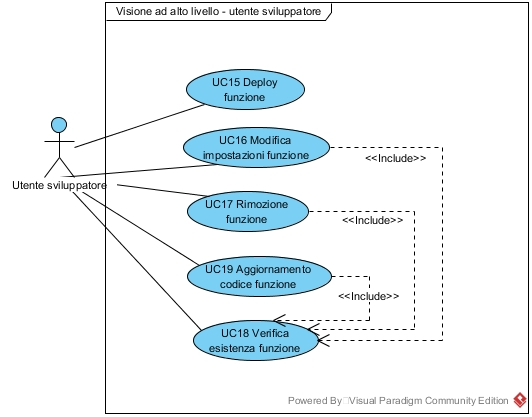
\includegraphics[width=\linewidth]{res/img/utenteSviluppatore.jpg}
	\caption{Diagramma visione ad alto livello - utente sviluppatore}
\end{figure}
\begin{itemize}
	\item \textbf{Attori primari:} Utente sviluppatore;
	\item \textbf{Descrizione:} l'utente che ha eseguito l'autenticazione a \textit{Etherless} mediante l'utenza \textit{Ethereum\glo} e, disponendo di una funzione JavaScript da rendere utilizzabile sulla piattaforma, ha accesso ai comandi dedicati agli utenti sviluppatori; 
	\item \textbf{Pre-condizioni:} l'utente ha eseguito l'accesso al sistema e e possiede una funzione JavaScript da caricare sulla piattaforma; 
	\item \textbf{Post-condizioni:} l'utente potrà eseguire i comandi messi a disposizione per gli utenti sviluppatori;
	\item \textbf{Scenario principale:} 
	\begin{enumerate}
		\item L'utente può eseguire il il deploy di una propria funzione JavaScript (UC15);
		\item L'utente può modificare le impostazione di una sua funzione presente nel sistema (UC16);
		\item L'utente può rimuovere una sua funzione presente nel sistema (UC17);
		\item L'utente può aggiornare il codice di una sua funzione presente nel sistema (UC19);
		\item L'utente può eseguire le operazioni descritte da UC16, UC17, UC18 solo se la funzione esiste all'interno della piattaforma (UC18).
	\end{enumerate}
\end{itemize}
\vspace{0.5cm}
\subsubsection{UC15 - Deploy\glo funzione}
\begin{figure}[h]
	\centering
	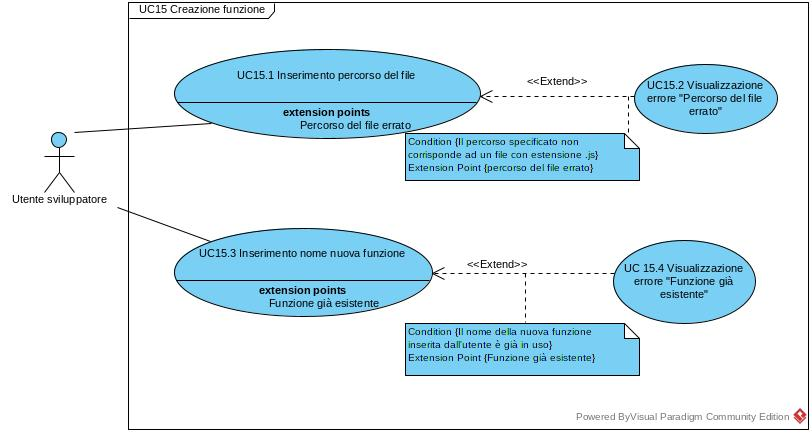
\includegraphics[width=\linewidth]{res/img/UC15.jpg}
	\caption{Diagramma UC15 - Deploy funzione}
\end{figure}
\begin{itemize}
	\item \textbf{Attori primari:} Utente sviluppatore;
	\item \textbf{Descrizione:} l'utente potrà eseguire il \textit{deploy\glo} di una propria funzione JavaScript su \textit{Etherless-server} rendendola disponibile a tutti gli utenti del servizio; 
	\item \textbf{Pre-condizioni:} l'utente possiede una funzione JavaScript sul proprio dispositivo;
	\item \textbf{Post-condizioni:} il sistema si occuperà di creare una nuova istanza su AWS Lambda con il nome specificato e rendere disponibile la sua esecuzione a tutti gli utenti di \textit{Etherless}. L'utente visualizzerà a schermo l'esito del comando;
	\item \textbf{Scenario principale:} 
	\begin{enumerate}
		\item L'utente tramite il comando \textit{"deploy\glos"} crea una nuova istanza della funzione su AWS Lambda;
		\item Il sistema visualizzerà su schermo l'esito dell'operazione.
	\end{enumerate}
\end{itemize}
\vspace{0.5cm}
\subsubsection{UC15.1 - Inserimento percorso del file}
\begin{itemize}
	\item \textbf{Attori primari:} Utente sviluppatore;
	\item \textbf{Descrizione:} l'utente potrà inserire tramite \textit{CLI\glo} il percorso del file JavaScript contenente la funzione da condividere su \textit{Etherless}; 
	\item \textbf{Pre-condizioni:} l'utente ha inserito tramite \textit{CLI\glo} il comando \textit{"deploy\glos"};
	\item \textbf{Post-condizioni:} l'utente ha inserito, a seguito del comando \textit{"deploy\glos"}, il nome da dare alla funzione che verrà caricata su \textit{Etherless};
	\item \textbf{Scenario principale:} l'utente inserisce il percorso del file contenente la funzione da caricare su \textit{Etherless};
	\item \textbf{Estensioni:} 
	\begin{itemize}
		\item \textbf{UC15.2}: il percorso inserito non corrisponde ad alcun file con estensione .js.
	\end{itemize}
\end{itemize}
\vspace{0.5cm}
\subsubsection{UC15.2 - Visualizzazione errore "Percorso del file errato"}
\begin{itemize}
	\item \textbf{Attori primari:} Utente sviluppatore;
	\item \textbf{Descrizione:} il sistema, a seguito dell'invio del comando contenente il percorso di un file non corretto, restituirà un errore. Il file della funzione deve avere l'estensione .js;
	\item \textbf{Pre-condizioni:}  l'utente invia il comando "create" seguito dal percorso del file Javascript sul proprio dispositivo e dal nome della funzione da caricare su \textit{Etherless};
	\item \textbf{Post-condizioni:} il sistema notificherà un errore tramite \textit{CLI\glo} che segnala la presenza di un percorso errato;
	\item \textbf{Scenario principale:} il sistema segnalerà all'utente un messaggio "Percorso del file errato".
\end{itemize}
\vspace{0.5cm}
\subsubsection{UC15.3 - Inserimento nome nuova funzione}
\begin{itemize}
	\item \textbf{Attori primari:} Utente sviluppatore;
	\item \textbf{Descrizione:} l'utente potrà specificare il nome della funzione che intende caricare e condividere su \textit{Etherless}. Il nome definito in questa fase sarà quello con il quale gli altri utenti potranno eseguire la funzione; 
	\item \textbf{Pre-condizioni:} l'utente ha inserito tramite \textit{CLI\glo} il comando \textit{"deploy\glos"} seguito dal percorso del file;
	\item \textbf{Post-condizioni:} l'utente ha inserito, a seguito del percorso del file, il nome della funzione che verrà caricata su \textit{Etherless};
	\item \textbf{Scenario principale:} l'utente inserisce il nome della funzione che vuole caricare su \textit{Etherless};
	\item \textbf{Estensioni:} 
	\begin{itemize}
		\item \textbf{UC15.4}: è già presente un'altra funzione in \textit{Etherless} con il nome inserito.
	\end{itemize}
\end{itemize}
\vspace{0.5cm}
\subsubsection{UC15.4 - Visualizzazione errore "Funzione già esistente"}
\begin{itemize}
	\item \textbf{Attori primari:} Utente sviluppatore;
	\item \textbf{Descrizione:} il sistema, a seguito dell'invio del comando, restituirà un errore "Funzione già esistente";
	\item \textbf{Pre-condizioni:}  l'utente invia il comando "create" seguito dal percorso del file Javascript sul proprio dispositivo e dal nome della funzione da caricare su \textit{Etherless};
	\item \textbf{Post-condizioni:} il sistema notificherà un errore tramite \textit{CLI\glo} che segnala la presenza di una funzione con lo stesso nome su \textit{Etherless};
	\item \textbf{Scenario principale:} il sistema segnalerà all'utente un messaggio "Funzione già esistente";
\end{itemize}
\vspace{0.5cm}
\subsubsection{UC16 - Modifica impostazioni funzione}
\begin{figure}[h]
	\centering
	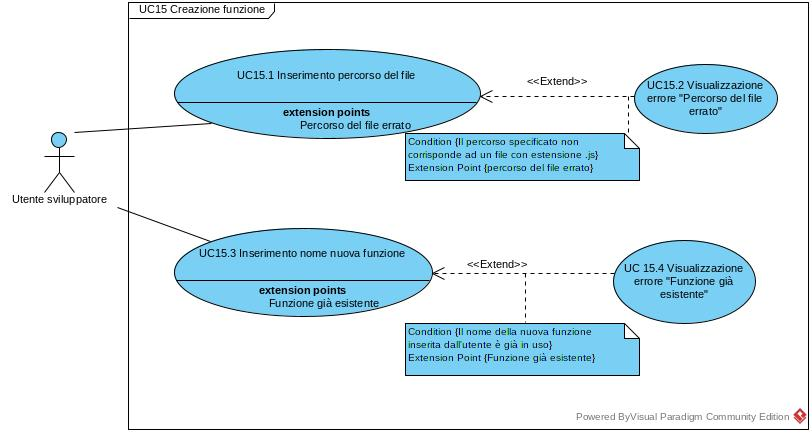
\includegraphics[width=\linewidth]{res/img/UC15.jpg}
	\caption{Diagramma UC16 - Modifica impostazioni funzione}
\end{figure}
\begin{itemize}
	\item \textbf{Attori primari:} Utente sviluppatore;
	\item \textbf{Descrizione:} l'utente potrà modificare alcune impostazioni della funzioni da rendere disponibili agli altri utenti di \textit{Etherless}; 
	\item \textbf{Pre-condizioni:} l'utente ha eseguito il \textit{"deploy\glos"} di almeno una funzione su \textit{Etherless};
	\item \textbf{Post-condizioni:} verranno modificate le impostazioni di una determinata funzione e saranno rese visibili agli altri utenti della piattaforma. L'utente visualizzerà a schermo l'esito del comando;
	\item \textbf{Scenario principale:} 
	\begin{enumerate}
		\item L'utente esegue la modifica delle impostazioni di una funzione mediante l'apposito comando. Avrà dunque la possibilità di modificarne:
		\begin{itemize}
			\item costo;
			\item descrizione;
			\item firma.
		\end{itemize}
		\item Il sistema visualizzerà su schermo l'esito dell'operazione effettuata.
	\end{enumerate}
	\item \textbf{Inclusioni:} 
	\begin{itemize}
		\item \textbf{UC18:} l'utente può modificare le impostazioni di una sua funzione solo se già presente in \textit{Etherless}.
	\end{itemize}	
\end{itemize}
\vspace{0.5cm}
\subsubsection{UC16.1 - Inserimento costo della funzione}
\begin{itemize}
	\item \textbf{Attori primari:} Utente sviluppatore;
	\item \textbf{Descrizione:} l'utente potrà inserire tramite \textit{CLI\glo} il costo da applicare ad una sua funzione. Un utente, per ciascuna esecuzione della funzionalità, dovrà pagare il prezzo impostato in questa fase. Una percentuale della somma dovuta all'utente sviluppatore verrà trattenuta da \textit{Ethereum\glo} per il mantenimento della piattaforma;
	\item \textbf{Pre-condizioni:} l'utente ha inserito tramite \textit{CLI\glo} il comando "set" seguito dal nome della funzione da lui caricata su \textit{Ethereum\glos};
	\item \textbf{Post-condizioni:} l'utente ha inserito, a seguito del nome della funzione di riferimento, il relativo costo;
	\item \textbf{Scenario principale:} l'utente inserisce il costo che vuole assegnare a una sua funzione presente su \textit{Etherless};
	\item \textbf{Estensioni:}
	\begin{itemize}
		\item \textbf{UC16.2}: il costo per l'esecuzione di una funzione non può essere 0 o inferiore.
		\item \textbf{UC19}: il nome della funzione non è tra quelle caricate dall'utente
	\end{itemize}
\end{itemize}

\vspace{0.5cm}
\subsubsection{UC16.2 - Visualizzazione errore "Costo non valido"}
\begin{itemize}
	\item \textbf{Attori primari:} Utente sviluppatore;
	\item \textbf{Descrizione:} il sistema, a seguito dell'invio del comando, restituirà un errore "Costo non valido" se il costo inserito risulta minore o uguale a 0;
	\item \textbf{Pre-condizioni:}  l'utente invia il comando "set" seguito dal nome della funzione da lui caricata su \textit{Ethereum\glos}, dal costo e dalla descrizione;
	\item \textbf{Post-condizioni:} il sistema notificherà un errore tramite \textit{CLI\glo} che segnala l'inserimento di un costo non accettabile;
	\item \textbf{Scenario principale:} il sistema segnalerà all'utente un messaggio "Costo non valido" per avere impostato un costo con valore negativo o nullo.
\end{itemize}
\vspace{0.5cm}
\subsubsection{UC16.3 - Inserimento descrizione della funzione}
\begin{itemize}
	\item \textbf{Attori primari:} Utente sviluppatore;
	\item \textbf{Descrizione:} l'utente potrà inserire tramite \textit{CLI} una descrizione per una funzione da lui caricata. Ciò consentirà ad un utente di conoscere dettagli della funzione non intuibili dalla sola segnatura; 
	\item \textbf{Pre-condizioni:} l'utente ha inserito tramite \textit{CLI\glo} il comando "set" seguito dal nome della funzione da lui caricata su \textit{Ethereum} e dal costo;
	\item \textbf{Post-condizioni:} l'utente ha inserito, a seguito del costo della funzione di riferimento, la relativa descrizione;
	\item \textbf{Scenario principale:} l'utente inserisce una breve descrizione per una sua funzione presente su \textit{Etherless};
	\item \textbf{Estensioni:} 
	\begin{itemize}
		\item \textbf{UC16.4}: la descrizione non può superare una lunghezza massima in caratteri.
	\end{itemize}
\end{itemize}
\vspace{0.5cm}
\subsubsection{UC16.4 - Visualizzazione errore "Descrizione troppo lunga"}
\begin{itemize}
	\item \textbf{Attori primari:} Utente sviluppatore;
	\item \textbf{Descrizione:} il sistema, a seguito dell'invio del comando, restituirà un errore "Descrizione troppo lunga" se la descrizione della funzione eccede il numero massimo di caratteri concessi;
	\item \textbf{Pre-condizioni:}  l'utente invia il comando "set" seguito dal nome della funzione da lui caricata su \textit{Ethereum}, dal costo e dalla descrizione;
	\item \textbf{Post-condizioni:} il sistema notificherà un errore tramite \textit{CLI\glo} che segnala l'inserimento della descrizione non accettabile;
	\item \textbf{Scenario principale:} il sistema segnalerà all'utente un messaggio "Descrizione troppo lunga" per avere impostato una descrizione che supera il numero consentito di caratteri.
\end{itemize}
\vspace{0.5cm}
\subsubsection{UC16.5 - Inserimento firma della funzione}
\begin{itemize}
	\item \textbf{Attori primari:} Utente sviluppatore;
	\item \textbf{Descrizione:} l'utente potrà inserire tramite \textit{CLI\glo} la firma di una propria funzione in formato stringa, in modo che un utente utilizzatore possa essere a conoscenza dei parametri richiesti;
	\item \textbf{Pre-condizioni:} l'utente ha inserito tramite \textit{CLI\glo} il comando "set" seguito dal nome della funzione da lui caricata su \textit{Ethereum\glos}, dal costo e dalla descrizione;
	\item \textbf{Post-condizioni:} l'utente ha inserito, a seguito della descrizione della funzione di riferimento, la relativa firma specificandone tipo di ritorno, numero e tipo dei parametri;
	\item \textbf{Scenario principale:} l'utente inserisce la firma di una sua funzione presente su \textit{Etherless}.
\end{itemize}

\vspace{0.5cm}
\subsubsection{UC17 - Deploy\glo funzione}
\begin{figure}[h]
	\centering
	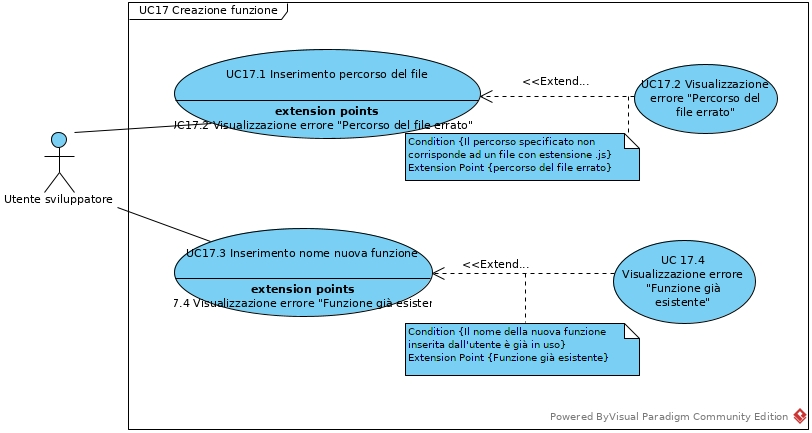
\includegraphics[width=\linewidth]{res/img/UC17.jpg}
	\caption{Diagramma UC17 - Deploy funzione}
\end{figure}
\begin{itemize}
	\item \textbf{Attori primari:} Utente sviluppatore;
	\item \textbf{Descrizione:} l'utente potrà eseguire il \textit{deploy\glo} di una propria funzione JavaScript su \textit{Etherless-server} rendendola disponibile a tutti gli utenti del servizio;
	\item \textbf{Pre-condizioni:} l'utente possiede una funzione JavaScript sul proprio dispositivo;
	\item \textbf{Post-condizioni:} il sistema si occuperà di creare una nuova istanza su AWS Lambda con il nome specificato e rendere disponibile la sua esecuzione a tutti gli utenti di \textit{Etherless}. L'utente visualizzerà a schermo l'esito del comando;
	\item \textbf{Scenario principale:}
	\begin{enumerate}
		\item L'utente tramite il comando \textit{"deploy\glos"} crea una nuova istanza della funzione su AWS Lambda;
		\item Il sistema visualizzerà su schermo l'esito dell'operazione.
	\end{enumerate}
\end{itemize}

\vspace{0.5cm}
\subsubsection{UC18 - Modifica impostazioni funzione}
\begin{figure}[h]
	\centering
	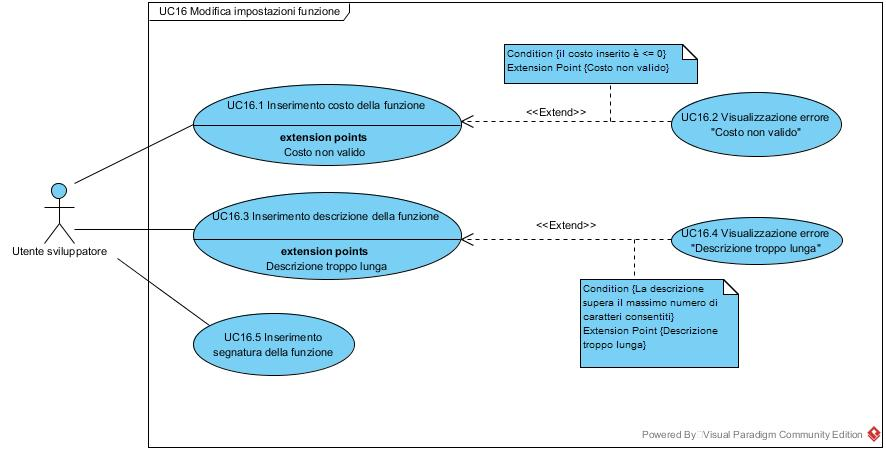
\includegraphics[width=\linewidth]{res/img/UC16.jpg}
	\caption{Diagramma UC18 - Modifica impostazioni funzione}
\end{figure}
\begin{itemize}
	\item \textbf{Attori primari:} Utente sviluppatore;
	\item \textbf{Descrizione:} l'utente potrà modificare alcune impostazioni della funzioni da rendere disponibili agli altri utenti di \textit{Etherless};
	\item \textbf{Pre-condizioni:} l'utente ha eseguito il \textit{"deploy\glos"} di almeno una funzione su \textit{Etherless};
	\item \textbf{Post-condizioni:} verranno modificate le impostazioni di una determinata funzione e saranno rese visibili agli altri utenti della piattaforma. L'utente visualizzerà a schermo l'esito del comando;
	\item \textbf{Scenario principale:}
	\begin{enumerate}
		\item L'utente esegue la modifica delle impostazioni di una funzione mediante l'apposito comando. Avrà dunque la possibilità di modificarne:
		\begin{itemize}
			\item costo;
			\item descrizione;
			\item firma.
		\end{itemize}
		\item Il sistema visualizzerà su schermo l'esito dell'operazione effettuata.
	\end{enumerate}
	\item\textbf{Estensioni:}
	\begin{itemize}
		\item \textbf{UC21}: il nome della funzione non è tra quelle caricate dall'utente.
	\end{itemize}
\end{itemize}

\vspace{0.5cm}
\subsubsection{UC18.1 - Inserimento costo della funzione}
\begin{itemize}
	\item \textbf{Attori primari:} Utente sviluppatore;
	\item \textbf{Descrizione:} l'utente potrà inserire tramite \textit{CLI\glo} il costo da applicare ad una sua funzione. Un utente, per ciascuna esecuzione della funzionalità, dovrà pagare il prezzo impostato in questa fase. Una percentuale della somma dovuta all'utente sviluppatore verrà trattenuta da \textit{Ethereum\glo} per il mantenimento della piattaforma;
	\item \textbf{Pre-condizioni:} l'utente ha inserito tramite \textit{CLI\glo} il comando "set" seguito dal nome della funzione da lui caricata su \textit{Ethereum\glos};
	\item \textbf{Post-condizioni:} l'utente ha inserito, a seguito del nome della funzione di riferimento, il relativo costo;
	\item \textbf{Scenario principale:} l'utente inserisce il costo che vuole assegnare a una sua funzione presente su \textit{Etherless};
	\item \textbf{Estensioni:}
	\begin{itemize}
		\item \textbf{UC18.2}: il costo per l'esecuzione di una funzione non può essere 0 o inferiore.
	\end{itemize}
\end{itemize}

\vspace{0.5cm}
\subsubsection{UC18.2 - Visualizzazione errore "Percorso del file errato"}
\begin{itemize}
	\item \textbf{Attori primari:} Utente sviluppatore;
	\item \textbf{Descrizione:} il sistema, a seguito dell'inserimento dell'invio del comando contenente il percorso di un file non corretto, restituirà un errore. Il file della funzione deve avere l'estensione .js;
	\item \textbf{Pre-condizioni:}  l'utente invia il comando "update" seguito dal nome della funzione da aggiornare e dal percorso del file JavaScript sul proprio dispositivo;
	\item \textbf{Post-condizioni:} il sistema notificherà un errore tramite \textit{CLI\glo} che segnala la presenza di un percorso errato;
	\item \textbf{Scenario principale:} il sistema segnalerà all'utente un messaggio "Percorso del file errato".
\end{itemize}

\vspace{0.5cm}
\subsubsection{UC19 - Aggiornamento codice funzione}
\begin{figure}[h]
	\centering
	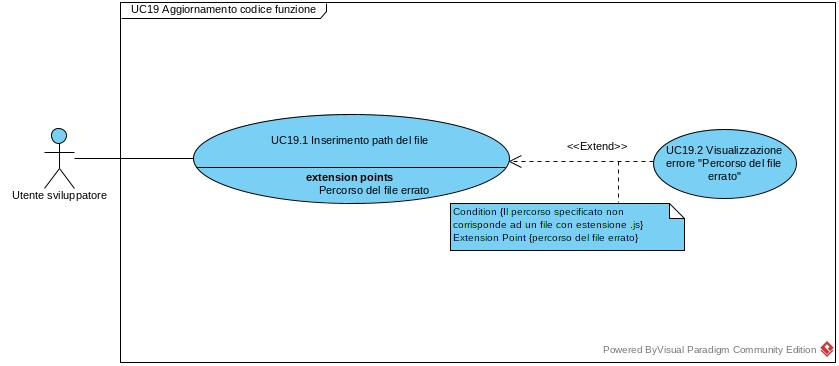
\includegraphics[width=\linewidth]{res/img/UC19.jpg}
	\caption{Diagramma UC19 - Aggiornamento codice funzione}
\end{figure}
\begin{itemize}
	\item \textbf{Attori primari:} Utente sviluppatore;
	\item \textbf{Descrizione:} l'utente potrà eseguire nuovamente il deploy di una sua funzione preesistente, aggiornandone il codice; 
	\item \textbf{Pre-condizioni:} l'utente possiede una funzione Javascript sul proprio dispositivo;
	\item \textbf{Post-condizioni:} il sistema si occuperà di aggiornare il codice della funzione da lui già condivisa su \textit{Etherless}. L'utente visualizzerà a schermo l'esito del comando;
	\item \textbf{Scenario principale:} 
	\begin{enumerate}
		\item L'utente tramite il comando "deploy" aggiorna il codice di una sua funzione;
		\item Il sistema visualizzerà su schermo l'esito dell'operazione.
	\end{enumerate}
\end{itemize}
\vspace{0.5cm}
\subsubsection{UC19.1 - Inserimento percorso del file}
\begin{itemize}
	\item \textbf{Attori primari:} Utente sviluppatore;
	\item \textbf{Descrizione:} l'utente potrà inserire tramite \textit{CLI\glo} il percorso del file Javascript contenente la funzione da modificare; 
	\item \textbf{Pre-condizioni:} l'utente ha inserito tramite \textit{CLI\glo} il comando "update" seguito dal nome della funzione di cui aggiornare il codice;
	\item \textbf{Post-condizioni:} l'utente ha inserito, a seguito del nome della funzione, il nuovo percorso del file.js;
	\item \textbf{Scenario principale:} l'utente inserisce il percorso del file per aggiornare il codice di una sua funzione presente su \textit{Etherless};
	\item \textbf{Estensioni:} 
	\begin{itemize}
		\item \textbf{UC19.2}: il percorso inserito non corrisponde ad alcun file con estensione .js.
	\end{itemize}
\end{itemize}
\vspace{0.5cm}
\subsubsection{UC19.2 - Visualizzazione errore "Percorso del file errato"}
\begin{itemize}
	\item \textbf{Attori primari:} Utente sviluppatore;
	\item \textbf{Descrizione:} il sistema, a seguito dell'inserimento dell'invio del comando contenente il percorso di un file non corretto, restituirà un errore. Il file della funzione deve avere l'estensione .js;
	\item \textbf{Pre-condizioni:}  l'utente invia il comando "update" seguito dal nome della funzione da aggiornare e dal percorso del file Javascript sul proprio dispositivo;
	\item \textbf{Post-condizioni:} il sistema notificherà un errore tramite \textit{CLI\glo} che segnala la presenza di un percorso errato;
	\item \textbf{Scenario principale:} il sistema segnalerà all'utente un messaggio "Percorso del file errato".
\end{itemize}
\vspace{0.5cm}
